\documentclass[15pt,journal]{IEEEtran}

\usepackage{algorithm}
\usepackage{algpseudocode}
\usepackage{hyperref}
\hypersetup{
    colorlinks=true,
    linkcolor=blue,
    filecolor=magenta,      
    urlcolor=blue,
    pdftitle={Overleaf Example},
    pdfpagemode=FullScreen,
    }
% *** CITATION PACKAGES ***
\usepackage[style=ieee]{biblatex} 
\bibliography{example_bib.bib}    %your file created using JabRef

% *** MATH PACKAGES ***
\usepackage{amsmath,bm}

% *** PDF, URL AND HYPERLINK PACKAGES ***
\usepackage{url}
% correct bad hyphenation here
\hyphenation{op-tical net-works semi-conduc-tor}
\usepackage{graphicx}  %needed to include png, eps figures
\usepackage{float}  % used to fix location of images i.e.\begin{figure}[H]

\begin{document}

% paper title
\title{\LARGE{ \textbf{ Indian Institute of Information Technology Vadodara(IIITV)}}\\ \LARGE{CS362 Artificial Intelligence Laboratory Report}}



\author{\Large{
\IEEEauthorblockN{$^{1}$ Bhatt Krutarth(201951041) \\$^{2}$ Bhimani Yash(201951042)\\ $^{3}$ Rakshilkumar Modi(201951124) \\$^{4}$ Zala Indravijaysinh(201951182) }
}%
}




% make the title area
\maketitle

% As a general rule, do not put math, special symbols or citations
% in the abstract or keywords.
\section{\large{\underline{Introduction}}}
In this lab report we have given an overview of the experiments, observation and results while performing 4 experiments. We have chosen experiment:
\begin{itemize}
    \item Week0:To be able to model a given problem in terms of state space search problem and solve the same using BFS/ DFS

    \item Week1 :To design a graph search agent and understand the use of a hash table, queue in state space search.
    \item Week3 : Non-deterministic Search - Simulated Annealing
    \item Week5: Game Playing Agent
    \item Week6: Understanding Bayesian Network
    \item Week10: Basics of data structure needed for state-space search tasks and use of random numbers required for MDP and RL
    \item Week11: Understanding Exploitation - Exploration in simple n-arm bandit reinforcement learning task, epsilon-greedy algorithm
    \item Week13:To understand the design of type-1 (Mamdani) Fuzzy expert system

\end{itemize}
We have performed the experiments on jupyter notebook for Python Code and RStudio for R. At the end of this report the GitHub repository link is also added.
\section{\large{\underline{WEEK 0}}}
To be able to model a given problem in terms of state space search problem and solve the same using BFS/ DFS
\subsection{In the rabbit leap problem, three east-bound rabbits stand in a line blocked by three west-bound rabbits. They are crossing a stream with stones placed in the east west direction in a line. There is one empty stone between them. The rabbits can only move forward one or two steps. They can jump over one rabbit if the need arises, but not more than that. Are they smart enough to cross each other without having to step into the water? 
}
\begin{figure}[H]%[!ht]
\begin {center}
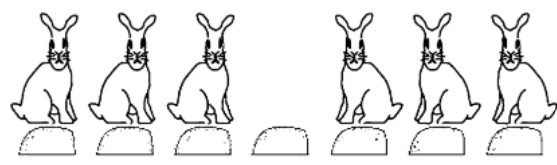
\includegraphics[width=0.48\textwidth]{images/rabbit .jpg}
\caption{Rabbit Leap Problem} % Caption change
\label{fig:ecg}
\end {center}
\end{figure}

In this problem the start state is the state shown in Fig 1. Our goal is to make the configuration in such a way that east-bound rabbits can to west side while the west-bound rabbit can go to east side, while maintaining the given conditions in the problem. One such solution can be:
Let Configuration be A,B,C,S,D,E,F(Here S represents space), Move D to S , then A,B,C,D,S,E,F. After this step move C to S so the configuration will be A,B,S,D,C,E,F. After this step move B to S so the configuration will be A,S,B,D,C,E,F , then move D to S, so configuration will be A,D,B,S,C,E,F. After this step move E to S, A,D,B,E,C,S,F. then move F to S, A,D,B,E,C,F,S, then move C to S A,D,B,E,S,F,C, then B to S A,D,S,E,B,F,C. similarly after continuing this process we can reach to position D,E,F,S,A,B,C which is our goal state.
\emph{Resources:} \href{https://www.thinkingapplied.com/frog_folder/frog.htm}{ Aesthetics of Problem Solving}

\subsection{The missionaries and cannibals problem is usually stated as follows. Three missionaries and three cannibals are on one side of a river, along with a boat that can hold one or two people. Find a way to get everyone to the other side without ever leaving a group of missionaries in one place outnumbered by the cannibals in that place. This problem is famous in AI because it was the subject of the first paper that approached problem-formulation from an analytical viewpoint. 
}

\begin{figure}[H]%[!ht]
\begin {center}
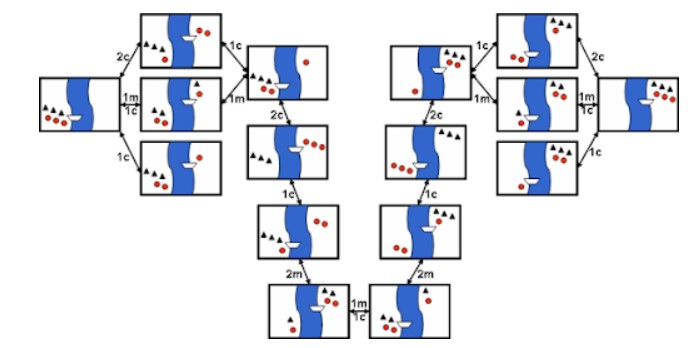
\includegraphics[width=0.48\textwidth]{images/cannibal.jpg}
\caption{Rabbit Leap Problem} % Caption change
\label{fig:ecg}
\end {center}
\end{figure}

For solving this, we use a 3-tuple (m, c, b) to represent the state of one side of the river, since the other side can be easily inferred. Here, m stands for the number of missionaries, c, the number of cannibals, and b, whether the boat is at this side of the river. Initially, we have the state (3, 3, 1) and the goal state should be (0, 0, 0).
Here, Actions are taken as

1m --- one missionary crosses the river

1c --- one cannibal crosses the river

2m ---- two missionaries cross the river

2c --- two cannibals cross the river

1m, 1c --- one missionary and one cannibal cross the river\\
\emph{Resources:} \href{https://cpentalk.com/201/missionaries-cannibals-problem-usually-missionaries-cannibals}{Missionaries-Cannibals}




\subsubsection{Model the problem as a state space search problem.  How large is the search space}
A state space is the set of all possible configurations of a system. It is a useful abstraction for reasoning about the behavior of a given system. The state space can be represented as a graph in which the vertices are states and the directed edges between them are actions. The approach for solving both the problem is explained above

\subsubsection{Solve the problem using BFS.  The optimal solution is the one with the fewest number of steps. Is the solution that you have acquired an optimal one? The program should print out the solution by listing a sequence of steps needed to reach the goal state from the initial state. } 
For implementing BFS we use Queue data structure that  works on 
first in, first out. BFS explores all nodes at one level before
proceeding to next level.So BFS find solution in optimal time.

In neither of the solution  BFS is optimal. In Rabbit leap problem total number of states are 44 state while in case of missionary and cannibal problem total number of state received is 22.For further explanation look for code in GitHub repository.

\subsubsection{Solve the problem using DFS.  The program should print out the solution by listing a sequence of steps needed to reach the goal state from the initial state}
In both the cases DFS gives optimal solution. In Rabbit leap problem total number of states are 23 state while in case of missionary and cannibal problem total number of state received is 20.For further explanation look for code in GitHub repository.

\subsubsection{Compare solutions found from BFS and DFS.  Comment on solutions. Also compare the time and space complexities of both.}

\underline{Comparison of solution BFS and DFS}
\begin{enumerate}
    \item DFS provides optimal solution than BFS by exploring less state.
    \item Solution depends on which how you are describing next possible state.
\end{enumerate}

In case of Missionary Cannibal problem branching factor = 5 while in case of Rabbit leap problem branching factor = 4
DFS \\
So Time complexity = {\bf{O(b{{$\bm{^{d}}$)}}}}\\
Space complexity = O(bd)

For BFS\\
Time complexity = {\bf{O(b{{$\bm{^{d}}$)}}}}\\
Space Complexity = {\bf{O(b{{$\bm{^{d}}$)}}}}

Here b is the branching factor and d is depth





\section{\large{\underline{WEEK 1}}}
 To design a graph search agent and understand the use of a hash table, queue in state space search.
 
\subsection{Write a pseudocode for a graph search agent. Represent the agent in the form of a flow chart. Clearly mention all the implementation details with reasons}

\underline{Answer:}

\begin{figure}[H]%[!ht]
\begin {center}
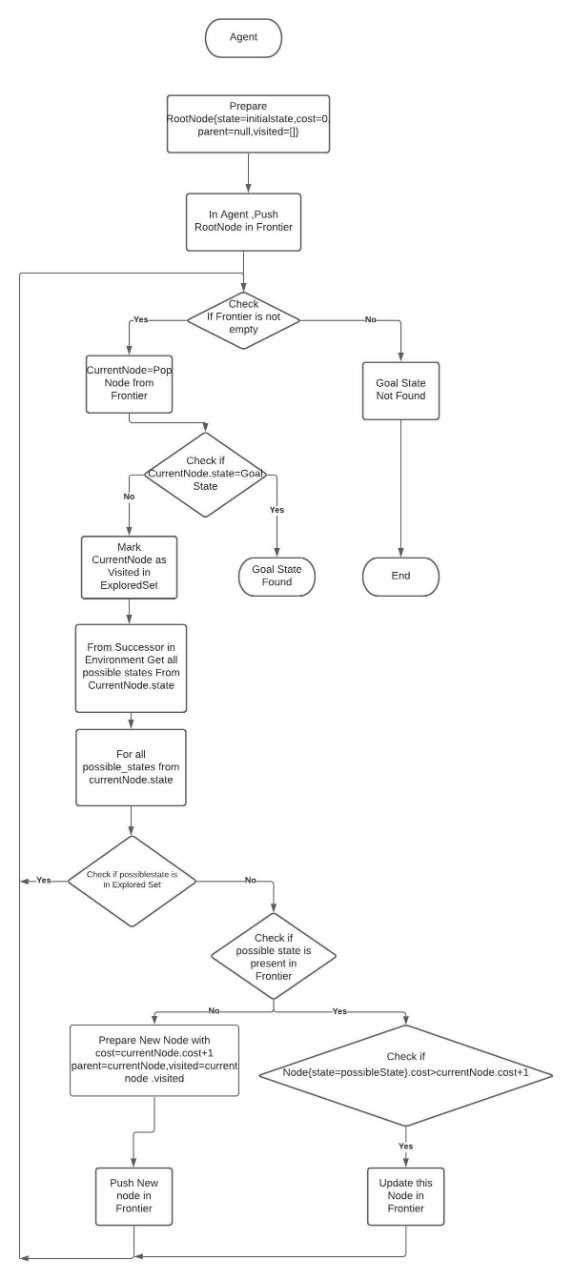
\includegraphics[width=0.48\textwidth]{images/Flowchart.jpeg}
\caption{Flow Chart of graph search agent} % Caption change
\label{fig:ecg}
\end {center}
\end{figure}

\begin{algorithm}
\caption{Graph Search Algorithm}\label{alg:cap}
\begin{algorithmic}[1]
\State Set environment for search by initializing start state, Goal state,hash map for explored nodes and Frontier queue
\State Initialize with the initial values of rootnode = start state,cost =0,parents,visited [] = in frontier
\While{Frontier is not empty }
    \State pop a element from frontier
    \If{CurrentNode.state =  Goalstate}
        \State Goal state reached
    \Else
        \State mark this state as Explored node in ExploredSet.
    \State $possible state \gets current state$
    \For{every state}
        \If{state not explored}
            \If{state present in frontier}
                \If{ new cost < previous cost}
                     \State Update the cost, parent, visited
                \EndIf
            \Else
                \State newNode with parent = currentNode
                \State cost = currentNode.cost+1
                \State visited = currentNode.visited+currentNode
            \EndIf
            \State If Goal not found, path not found
        \EndIf
    \EndFor
    \EndIf           
\EndWhile
\end{algorithmic}
\end{algorithm}




The {$8\-Puzzle$} has a matrix of 3X3 in which numbers from 1 to 8 are arranged randomly with an empty space . In the given figure the start state is [[7,2,4][5,0,6][8,3,1]] where 0 is represented as the blank space , we need to reach the final state [[0,1,2][3,4,5][6,7,8]] by moving the tiles

In case of {$8\-Puzzle$} the Start and  Goal state are as follows:.


\begin{figure}[H]%[!ht]
\begin {center}
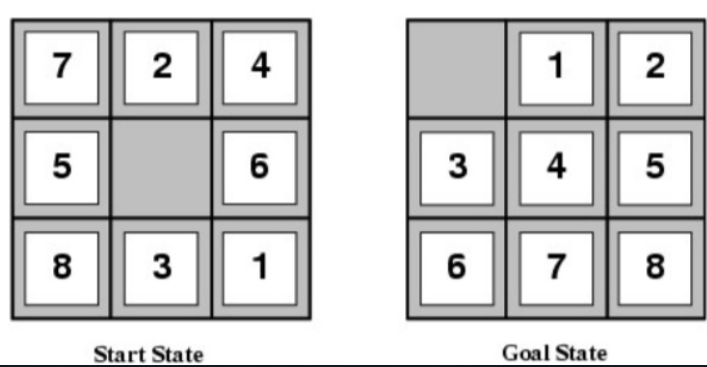
\includegraphics[width=0.48\textwidth]{images/8 puzzle.png}
\caption{Start state and Goal state of 8-Puzzle problem} % Caption change
\label{fig:ecg}
\end {center}
\end{figure}





 % line change mate \\

\subsection{Write a collection of functions imitating the environment for 8-Puzzle.}

\underline{Answer:}
Environment for 8 puzzle includes current state visited state , path traversed to reach the current node and cost for reaching to the goal state 
\emph{Function}\\
{\bf{check()}}: If the current state is goal state\\
{\bf{validate()}}: check if it is possible to move futhur or not\\
{\bf{getnext()}}:return next possible state\\


\subsection{Describe what is Iterative Deepening Search ?}

\underline{Answer:}
Iterative deepening search is search strategy used with depth first search(DFS).It does a series of depth first searches with increasing depth bounds(in every cycle it perfoms DFS with bound incremented by one)  same way as that breadth first search(BFS), but the only difference is that BFS stores all nodes in memory, while iterative-deepening does it by repeating the previous layers, thereby saving memory at the cost of more time.Therefore memory requirements grows linearly with depth.The time complexity of iterative deepening is same as dfs i.e. {\bf{O(b{{$\bm{^{d}}$)}}}} where b is the branching factor and d is the depth . The space complexity is {\bf{O(bd)}}.

\begin{figure}[H]%[!ht]
\begin {center}
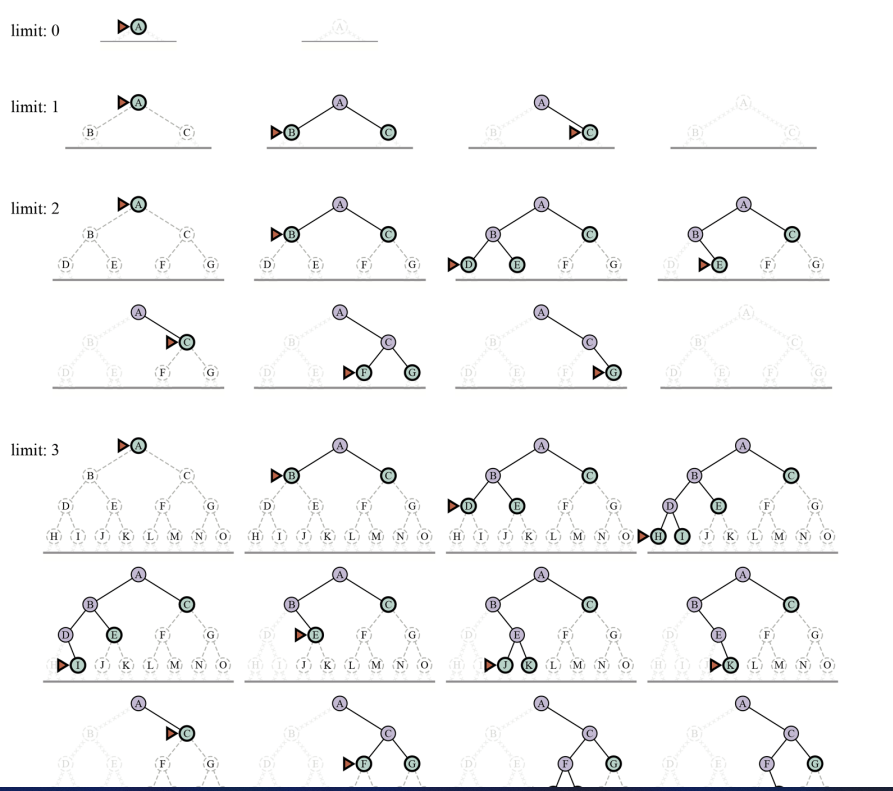
\includegraphics[width=0.48\textwidth]{images/ids.png}
\caption{Iterative Deepening Search} % Caption change
\label{fig:ecg}
\end {center}
\end{figure}

    
\subsection{Considering the cost associated with every move to be the same (uniform cost), write a function which can backtrack and produce the path taken to reach the goal state from the source/ initial state}

\underline{Answer:}

Please refer to the code for given in github repository


\subsection{Generate Puzzle-8 instances with the goal state at depth “d”.}

\underline{Answer:}

For generating puzzle 8 instances with goal state at depth "d". We have to explore each possible states from initial function in order to reach the goal state. For implementation refer to the code


\subsection{Prepare a table indicating the memory and time requirements to solve Puzzle-8 instances (depth “d”) using your graph search agent.}

\underline{Answer:}
\begin{table}[!ht] %[H]
\centering


\begin{tabular}{| c | c | c |}
\hline
Depth  &  Space  & time \\
\hline 
1 & 12288 &  0.002992868423 \\
\hline
2 & 16384 & 0.0059845 \\
\hline
3 & 24576 &  0.01897954 \\
\hline
4 & 98304 &  0.0446937084 \\
\hline
5 & 98304 &  0.097214698 \\
\hline
6 & 163840 &  0.1397825428 \\
\hline
7 & 233472 &  0.2627568244 \\
\hline
8 & 360448 &  0.345679283 \\

\hline
\end{tabular}

\label{table:Exps}
\caption{Latitude and Longitude of the Places of Rajasthan.}
\end{table}



\newpage
\section{\large{\underline{WEEK 3}}}
Non-deterministic Search | Simulated Annealing

\subsection{Travelling Salesman Problem (TSP) is a hard problem, and is simple to state.  Given a  graph in which the nodes are locations of cities, and edges are labelled with the cost of travelling between cities,  find a cycle containing each city exactly once, such that the total cost of the tour is as low as possible.}

\underline{Answer:}
Travelling Salesman Problem is popularly  known as TSP problem. In this problems like "Given a list of cities and the distances between each pair of cities, what is the shortest possible route that visits each city exactly once and returns to the origin city?" arises. It is an NP-hard problem in combinatorial optimization
Solution to Travelling salesman problem:
\subsubsection{Dynamic Programming(DP)}
The dynamic programming or DP method guarantees to find the best answer to TSP. However, its time complexity would exponentially increase with the number of cities. The time complexity with the DP method asymptotically equals N{$^{2}$} x 2{$^{N}$} where N is the number of cities
\subsubsection{Based on Euclidean distance} 
Let,

No. of cites = N
\\Total no of states = N!
\\here a city(i) is assumed to be present in x-y plane have coordinates = \((x {_{i}},y {_{i}})\).
\\\(D{_{i,j}}\) = Distance matrix of N x N which has the Euclidean distance between each city. Here a city is chosen through random permutation. Here we have to minimize the distance between cities and also find minimum distance between the origin and destination using the given equation :

\begin{equation}
  min.f(n) = \sum_{i=1}^{N-1}d(x {_{i}},x {_{i+1}}) + d(x {_{n}},x {_{1}})
    \label{equation:Tour Calculation Function}
\end{equation}

\subsubsection{Using Simulated Annealing}
Here we apply stimulated annealing approach to solve tsp,as it provides an optimal global solution to the given problem.The fundamental idea is to accept moves resulting in solutions of worse quality than the current solution in order to escape from local Minima. The probability of accepting such a move is decreased during the search through parameter temperature. SA algorithm starts with an initial solution x , and candidate solution y is then generated (either randomly or using some pre-specified rule) from the neighbourhood of x. The Metropolis acceptance criterion, which models how a thermodynamic system moves from one state to another state in which the energy is being minimized, is used to decide whether to accept y or not. The candidate solution y is accepted as the current solution x based on the acceptance probability:


\begin{equation}
   p = 
  \begin{cases}
     1 & \text{$if         (f(y) \leq f(x))$} \\
    e{{^{-(f(y)-f(x))/t}}} & \text{$otherwise$}
  \end{cases}
  \label{equation:Metropolis Acceptance Criterion}
\end{equation}


Here t is the controlling parameter which plays an important role in computing the probability.Initially the t value is high and the process moves further in order to get the minimum cost we keep on decreasing the t by 0.1 after every iteration.


\subsection{For the state of Rajasthan, find out at least twenty important tourist locations.  Suppose your relatives are about to visit you next week.  Use Simulated Annealing to plan a cost effective tour of Rajasthan.  It is reasonable to assume that the cost of travelling between two locations is proportional to the distance between them.}
\underline{Answer:}
Here we have taken twenty different places of  Rajasthan and for calculating the distance, we first gathered there latitude and longitude for calculating the distance between the place. The gathered latitude and longitude of each place is shown in the table given below:


\begin{table}[!ht] %[H]
\centering

\begin{tabular}{| c | c | c | c |}
\hline
Sr.no &  City & Latitude($N^{\circ}$) & Longitude( $E^{\circ}$) \\
\hline 
1 & Udaipur &  24.6 & 73.1 \\
\hline
2 & Jaisalmer &  26.9 & 70.9 \\
\hline
3 & Ganganagar &  29.9 & 73.8 \\
\hline
4 & Ajmer &  26.4 & 74.6 \\
\hline
5 & Jaipur &  26.9 & 75.7 \\
\hline
6 & Chittaurgarh &  24.8 & 74.6 \\
\hline
7 & Alwar &  27.5 & 76.6 \\
\hline
8 & Jodhpur &  26.2 & 73.0 \\
\hline
9 & Dungarpur &  23.8 & 73.7 \\
\hline
10 & Ranthambore &  26.0 & 76.5 \\
\hline
11 & Pushkar &  26.4 & 74.5 \\
\hline
12 & Kota &  25.2 & 75.8 \\
\hline
13 & Bundi &  25.4 & 75.6 \\
\hline
14 & Pali &  25.7 & 73.3 \\
\hline
15 & Kumbalgarh &  25.1 & 73.5 \\
\hline
16 & Bikaner &  28.0 & 73.3 \\
\hline
17 & Abu &  24.5 & 72.7 \\
\hline
18 & Ranakpur &  25.1 & 73.4 \\
\hline
19 & Nathdwara &  24.9 & 73.8 \\
\hline
20 & Fatehpur &  25.9 & 80.7 \\
\hline
\end{tabular}

\label{table:Exps}
\caption{Latitude and Longitude of the Places of Rajasthan.}
\end{table}

The distance between two places from given latitude and longitude can be found using Haversine-formula: \\
\emph{Resources:} \href{https://www.researchgate.net/publication/282314348_Landmark_based_shortest_path_detection_by_using_A_Algorithm_and_Haversine_Formula}{Harversine Formula}
\begin{equation}
 \resizebox{.9\hsize}{!} {  d = 2r\sin^{-1}{\sqrt{sin^2(\frac{N {_{2}} - N{_{1}}}{2})+  cos(N{_{2}})cos(N{_{1}})sin^2(\frac{E {_{2}} - E{_{1}}}{2})}}
  }
  \label{equation:Haversine-Formula}
\end{equation}





\begin{figure}[H]%[!ht]
\begin {center}
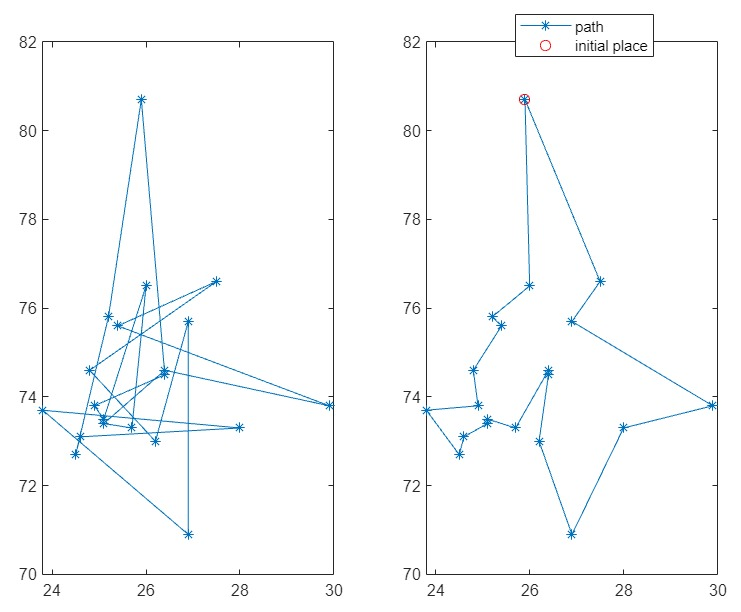
\includegraphics[width=0.45\textwidth]{images/tsp.jpeg}
\caption{ Graphs showing difference between Initial travelling without simulated annealing and travelling with simulated annealing } 
\label{fig:ecg}
\end {center}
\end{figure}

After finding the distances from the Haversine-Formula we obtain distance between every cities


\begin{figure}[H]%[!ht]
\begin {center}
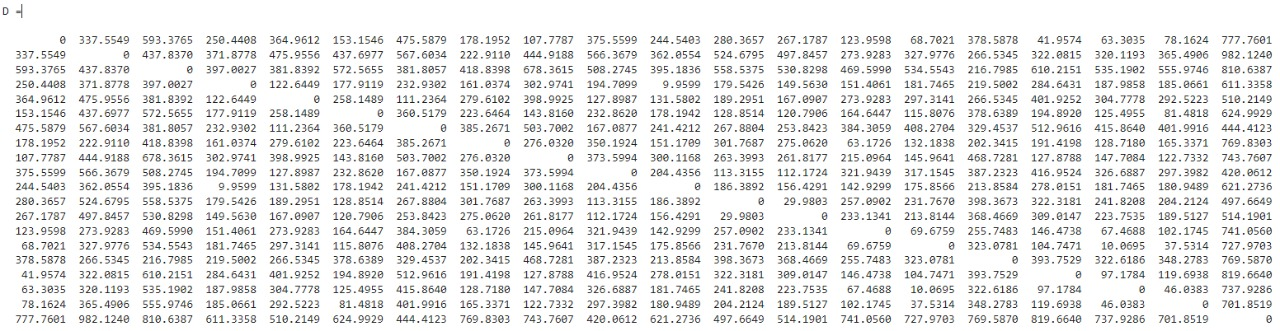
\includegraphics[width=0.48\textwidth]{images/tsp2.jpeg}
\caption{Distance  matrix  cities} % Caption change
\label{fig:ecg}
\end {center}
\end{figure}

Total distance cost = 3033.9 {\bf{kms}}.\\
Places traversed in the following manner : \\ Fatehpur,Alwar,Jaipur,Ganganagar,Bikaner,Jaisalmer,Jodhpur,Nathwara,
Chittaurgarh,Bundi,Kota,Ranthambore.



\subsection{An interesting problem domain with TSP instances:
VLSI: http://www.math.uwaterloo.ca/tsp/vlsi/index.html\#XQF131
(Attempt at least five problems from the above list and compare your results.)
}

\underline{Answer:} 
\subsubsection{\bf{Board 1}}
NAME: xqf131
COMMENT : Bonn VLSI data set with 131 points
COMMENT : Uni Bonn, Research Institute for Discrete Math
COMMENT : Contributed by Andre Rohe
TYPE : TSP
DIMENSION : 131
$EDGE\_WEIGHT\_TYPE$ : $EUC\_2D$


\begin{figure}[H]%[!ht]
\begin {center}
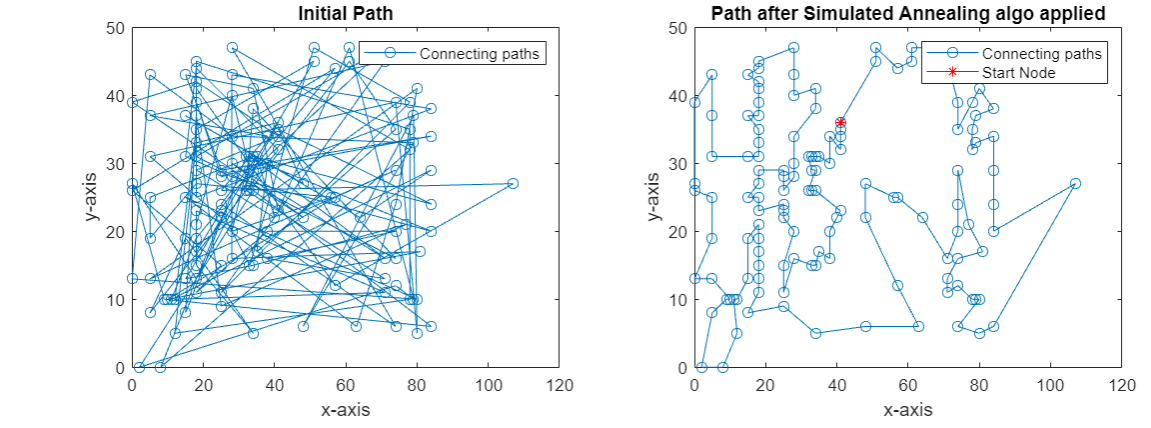
\includegraphics[width=0.48\textwidth]{images/tsp36.png}
\caption{Graphs showing difference between Initial travelling without simulated annealing and travelling with simulated annealing} % Caption change
\label{fig:ecg}
\end {center}
\end{figure}


\subsubsection{\bf{Board 2}}
NAME : xqg237
COMMENT : Bonn VLSI data set with 237 points
COMMENT : Uni Bonn, Research Institute for Discrete Math
COMMENT : Contributed by Andre Rohe
TYPE : TSP
DIMENSION : 237
$EDGE\_WEIGHT\_TYPE$ : $EUC\_2D$

\begin{figure}[H]%[!ht]
\begin {center}
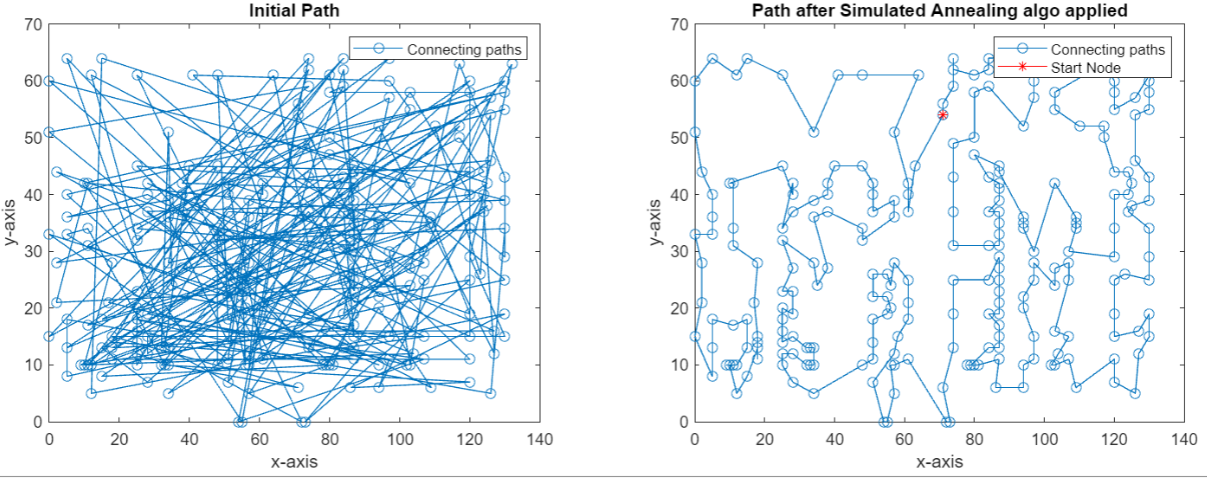
\includegraphics[width=0.48\textwidth]{images/_b2.PNG}
\caption{Graphs showing difference between Initial travelling without simulated annealing and travelling with simulated annealing} % Caption change
\label{fig:ecg}
\end {center}
\end{figure}

\subsubsection{\bf{Board 3}}
NAME : pbl395
COMMENT : Bonn VLSI data set with 395 points
COMMENT : Uni Bonn, Research Institute for Discrete Math
COMMENT : Contributed by Andre Rohe
TYPE : TSP
DIMENSION : 395
$EDGE\_WEIGHT\_TYPE : EUC\_2D$
$NODE\_COORD\_SECTION$

\begin{figure}[H]%[!ht]
\begin {center}
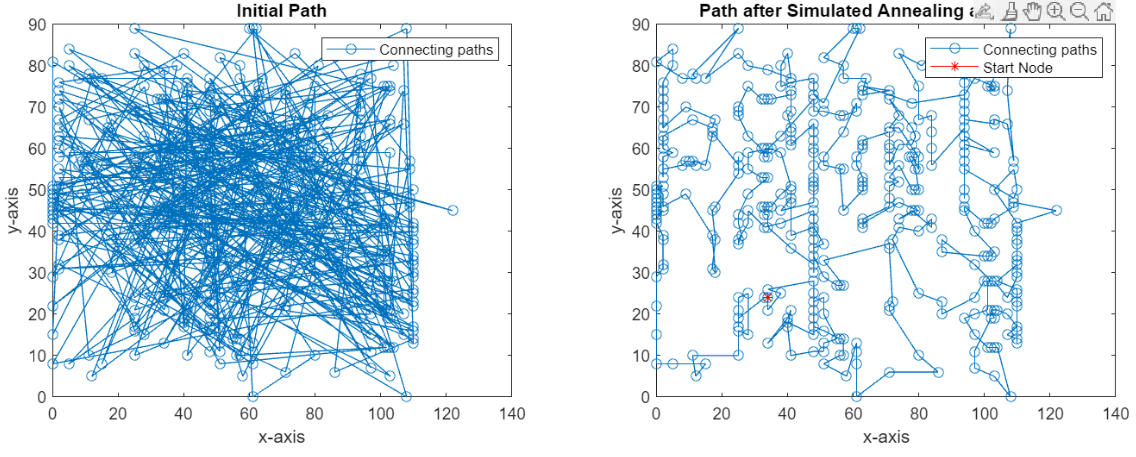
\includegraphics[width=0.48\textwidth]{images/_b3.PNG}
\caption{Graphs showing difference between Initial travelling without simulated annealing and travelling with simulated annealing} % Caption change
\label{fig:ecg}
\end {center}
\end{figure}

\subsubsection{\bf{Board 4}}
NAME : bcl380
COMMENT : Bonn VLSI data set with 380 points
COMMENT : Uni Bonn, Research Institute for Discrete Math
COMMENT : Contributed by Andre Rohe
TYPE : TSP
DIMENSION : 380
$EDGE\_WEIGHT\_TYPE : EUC\_2D$
$NODE\_COORD\_SECTION$


\begin{figure}[H]%[!ht]
\begin {center}
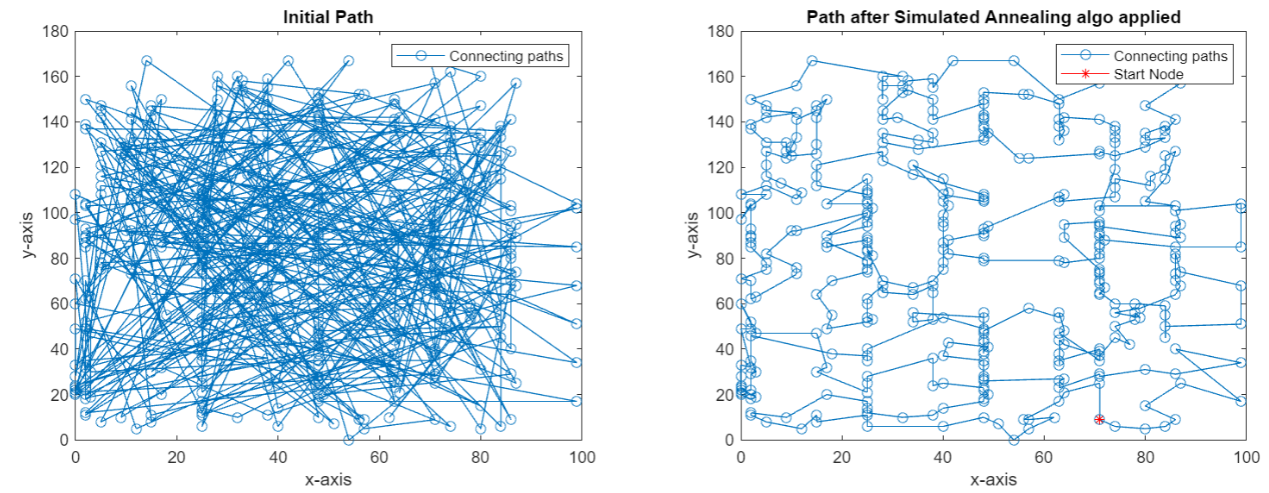
\includegraphics[width=0.48\textwidth]{images/_b4.PNG}
\caption{Graphs showing difference between Initial travelling without simulated annealing and travelling with simulated annealing} % Caption change
\label{fig:ecg}
\end {center}
\end{figure}

\subsubsection{\bf{Board 5}}
NAME : pbk411
COMMENT : Bonn VLSI data set with 411 points
COMMENT : Uni Bonn, Research Institute for Discrete Math
COMMENT : Contributed by Andre Rohe
TYPE : TSP
DIMENSION : 411
$EDGE\_WEIGHT\_TYPE : EUC\_2D$
$NODE\_COORD\_SECTION$

\begin{figure}[H]%[!ht]
\begin {center}
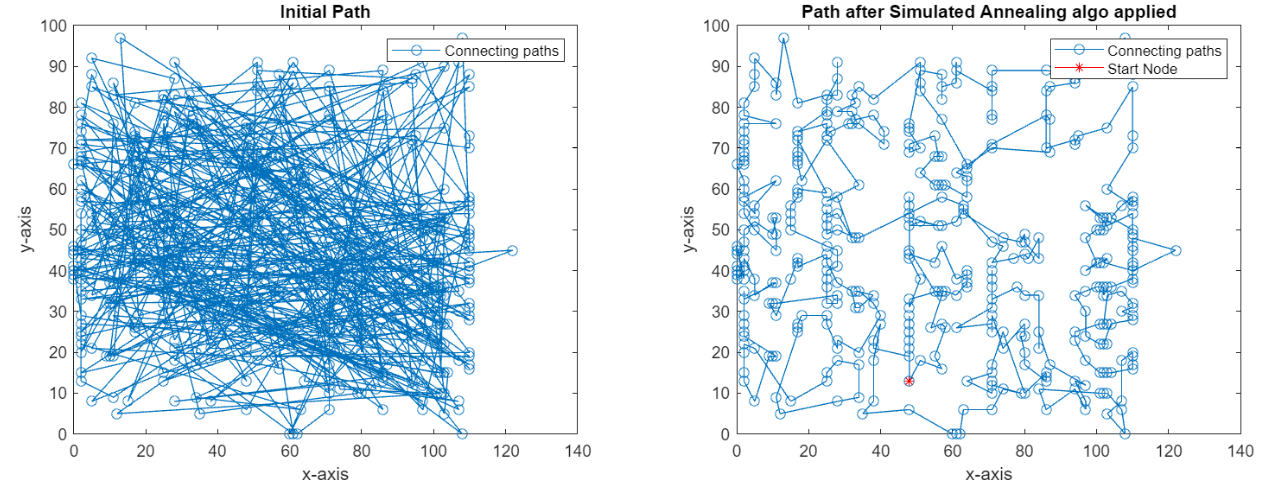
\includegraphics[width=0.48\textwidth]{images/_b5.PNG}
\caption{Graphs showing difference between Initial travelling without simulated annealing and travelling with simulated annealing} % Caption change
\label{fig:ecg}
\end {center}
\end{figure}


 
 %%%%%%%%%%%%%%%%%%%%%%%%%%%%

\section{\large{\underline{WEEK 5}}}
Game Playing Agent | Minimax | Alpha-Beta Pruning
Systematic adversarial search can lead to savings in terms of pruning of sub-trees resulting in lesser node evaluations
\subsection{What is the size of the game tree for Noughts and Crosses? Sketch the game tree.}
\underline{Answer:} 
Noughts and crosses(tic-Tac-Toe) is a interesting game which require two players. Each player has to play alternatively. It has 3X3 Empty board which has to filled by 'X' and 'O'. Game continues till either of the player wins or the game draws. Let's suppose Player 1 starts the game so it has 9 choices of filling the box(assuming he will be fill 'X') which we can consider as depth 1, after player 1's chance Player 2 will have to fill 'O' in 8 possible choices. Then again Player1 gets chance to fill out of 7 choices, and this continues till a player wins or the game draws. For wining the game either following conditions must be satisfied:
\begin{itemize}
    \item A row has same character i.e complete row has Use recurrence to show that under perfect ordering of leaf nodes, the alpha-beta pruning time complexity is O($b^{m/2}$), where b is the effective branching factor and m is the depth of the tree.to be either ('X' or 'O')
    \item A Column has same character i.e complete column has to be either ('X' or 'O')
    \item Either of the two diagonals have same character i.e complete diagonal has to be either ('X' or 'O')
\end{itemize}
So, Total possible states are 9! = 9x8x7x6x5x4x3x2x1 = 362880 states

\begin{figure}[H]%[!ht]
\begin {center}
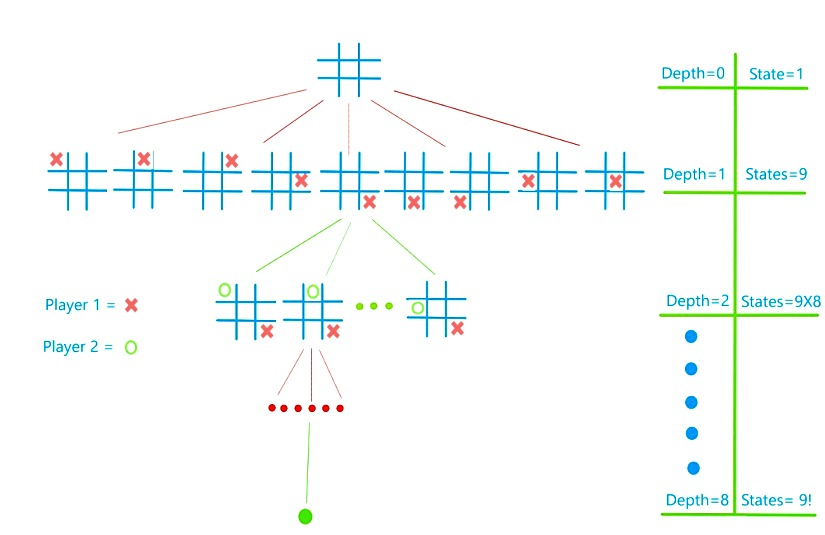
\includegraphics[width=0.45\textwidth]{images/minimax.png}
\caption{Tic-Tac-Toe game tree} 
\label{fig:ecg}
\end {center}
\end{figure}    
    

\subsection{Read about the game of Nim (a player left with no move losing the game). For the initial configuration of the game with three piles of objects as shown in Figure, show that regardless of the strategy of player-1, player-2 will always win. Try to explain the reason with the MINIMAX value backup argument on the game tree.}



\begin{figure}[H]%[!ht]
\begin {center}
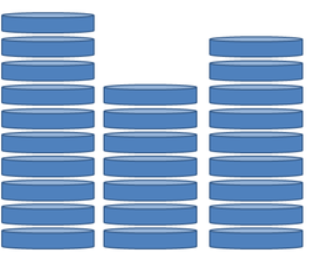
\includegraphics[width=0.45\textwidth]{images/Nim2.png}
\caption{ Hill Climbing with bdla Score} 
\label{fig:ecg}
\end {center}
\end{figure}

\underline{Answer:}
Game of Nim consists of 'n' piles where each pile contains i number of nims such that
\begin{equation}
   1 \leq i \leq n
    \label{equation: No of Nim }
\end{equation}

The player to pick the last nim is going to win the game

The winning in the Nim game depends on the two factor:
\begin{itemize}
    \item One who starts the game
    \item Initial configuration of game
\end{itemize}

Here with observation, if initial configuration of the Nims i.e if the XOR sum of the no. of the Nims is non-zero then who starts the game first will definitely lose. Here in the question starting configuration is [7,9,10] whose XOR is $4 \neq 0$ , hence even if player 1 has the strategy of winning the game he will definitely lose.


\subsection{Implement MINIMAX and alpha-beta pruning agents. Report on number of evaluated nodes for Noughts and Crosses game tree.}
\underline{Answer:} 
\emph{number of different states explored during finding of best move for a state in Minimax algorithm:} 29
\begin{figure}[H]%[!ht]
\begin {center}
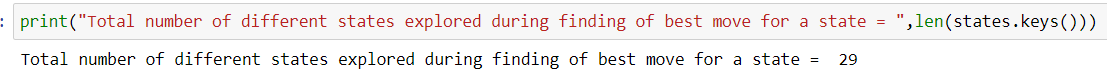
\includegraphics[width=0.48\textwidth]{images/Minimax outp.png}
\caption{} % Caption change
\label{fig:ecg}
\end {center}
\end{figure}
\emph{number of different states explored during finding of best move for a state in alpha-beta algorithm:} 12
\begin{figure}[H]%[!ht]
\begin {center}
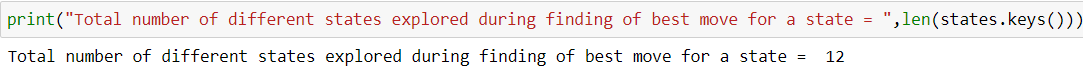
\includegraphics[width=0.48\textwidth]{images/alpha.png}
\caption{} % Caption change
\label{fig:ecg}
\end {center}
\end{figure}

\subsection{Use recurrence to show that under perfect ordering of leaf nodes, the alpha-beta pruning time complexity is O($b^{m/2}$), where b is the effective branching factor and m is the depth of the tree.}
\underline{Answer:} 
The time complexity of Minimax algorithm is O($b^{m}$) which can reduced by without checking each node. The technique of reduction in time complexity is called pruning. This involves two threshold parameters alpha and beta, thus this is also called alpha-beta pruning.

To determine exact value of a state, we need the exact value of one of its children and bounds on the rest of the children.For determining a bound of state's value, exact value of one of its children must be known.\\
Let S(k) be the minimum number of states to be considered k ply from a given state for knowing the exact value of the state. Similarly let R(k) be the minimum number of states to be considered k ply from a given state when we need to know a bound on the state's value.Let b be the branching factor. Thus,
\begin{equation}
   S(k) = S(k-1)+(b-1)R(k-1)
   \label{equation:  } 
\end{equation}



i.e., the exact value of one child and bounds on the rest,and 
\begin{equation}
   R(k) = S(k-1)
    \label{equation:  }
\end{equation}

i.e., the exact value of one child. The base is S(0) = R(0) = 1. Note, for fig, this gives S(3) = $b^{2}$ + b -1 = 11 for b = 3

when we expand the recursive equation, we get:\\
 S(k) = S(k-1)+(b-1)R(k-1)\\
       = (S(k-2)+(b-1)R(k-2)) + (b-1)S(k-2)\\
       = bS(k-2)+ (b-1)R(k-2)\\
      = bS(k-2) + (b-1)S(k-3)
  
It is obvious that S(k-3)<S(k-2),so:
S(k) < (2b-1)S(k-2)
     < 2bS(k-2)
     
That is, the branching factor every two levels is less than 2b, which means the effective branching factor is less than $\sqrt{2b}$.

So, for even k, we derive {{${S(k) \leq {($\sqrt{2b}$)^k}}$}}, which is not too far off the asymptotic upper bound of {{$($\sqrt{b}+\frac{1}{2}$) ^{k+1}$}}\\

%% Fault thik karbo %%%%%%%%%%%%%%%%%5

In effect, alpha-beta pruning can nearly double the depth that a game tree can be searched in comparison to straightforward minimax.\\

\emph{Resources:} \href{http://www.cs.utsa.edu/~bylander/cs5233/a-b-analysis.pdf}{a-b-analysis}



\section{\large{\underline{WEEK 6}}}

Understand the graphical models for inference under uncertainty, build Bayesian Network in R, Learn the structure and CPTs from Data, naive Bayes classification with dependency between features.

\subsection{Consider grades earned in each of the courses as random variables and learn the dependencies between courses.}

\underline{Answer:} 
Using the hill Climbing greedy search function 'hc' of the bnlearn package several different bayesian network based on scores have been generated.

\begin{figure}[H]%[!ht]
\begin {center}
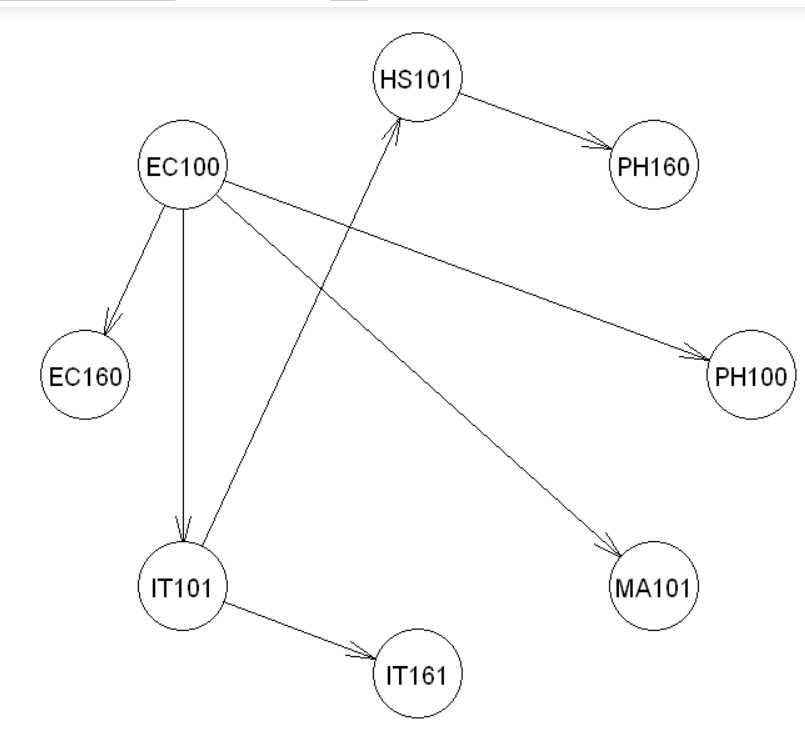
\includegraphics[width=0.48\textwidth]{images/Bayesian_aic.png}
\caption{Hill Climbing with aic Score} % Caption change
\label{fig:ecg}
\end {center}
\end{figure}

\subsubsection{Using {{\bf{'aic'}}} score}

MODEL: There are 7 dependencies between each subject which can seen from the above fig. using aic score and the dependencies are 
[EC100][EC160|EC100][IT101|EC100]
[MA101|EC100][PH100|EC100][IT161|IT101]
[HS101|IT101][PH160|HS101]



\subsubsection{Using {{\bf{'bdla'}}} score}
\begin{figure}[H]%[!ht]
\begin {center}
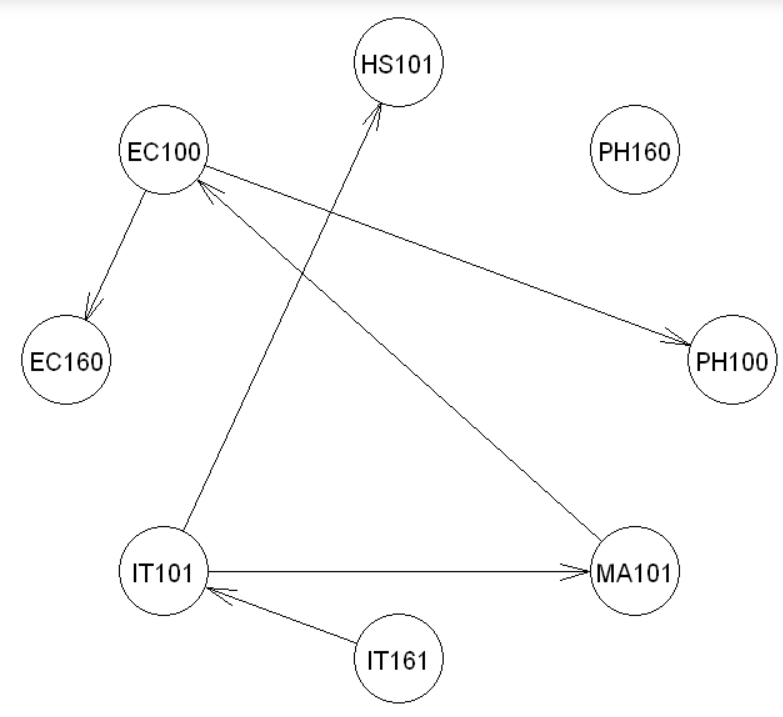
\includegraphics[width=0.48\textwidth]{images/Bayesian_bdla.png}
\caption{Hill Climbing with bdla Score} % Caption change
\label{fig:ecg}
\end {center}
\end{figure}
MODEL: There are 6 dependencies between each subject which can seen from the above fig. using bdla score and the dependencies are  [IT161][PH160][IT101|IT161][MA101|IT101]
[HS101|IT101][EC100|MA101][EC160|EC100]
[PH100|EC100].


\subsubsection{Using {{\bf{'bic'}}} score}
\begin{figure}[H]%[!ht]
\begin {center}
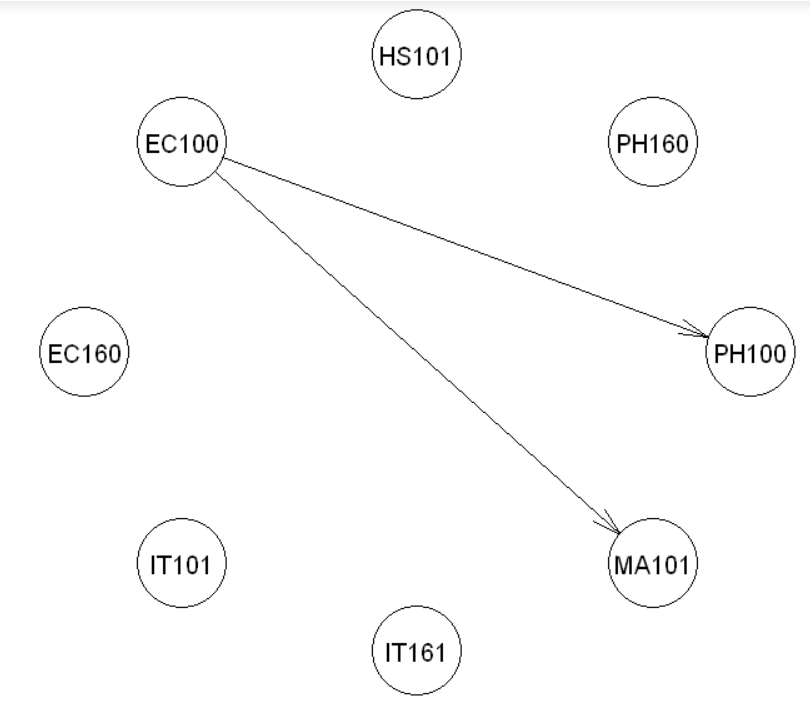
\includegraphics[width=0.48\textwidth]{images/Bayesian_bic.png}
\caption{Hill Climbing with bic Score} % Caption change
\label{fig:ecg}
\end {center}
\end{figure}

MODEL: There are 2 dependencies between each subject which can seen from the above fig. using bic score and the dependencies are
[EC100][EC160][IT101][IT161][PH160]
[HS101][MA101|EC100][PH100|EC100].


\subsubsection{Using {{\bf{'k2'}}} score}

\begin{figure}[H]%[!ht]
\begin {center}
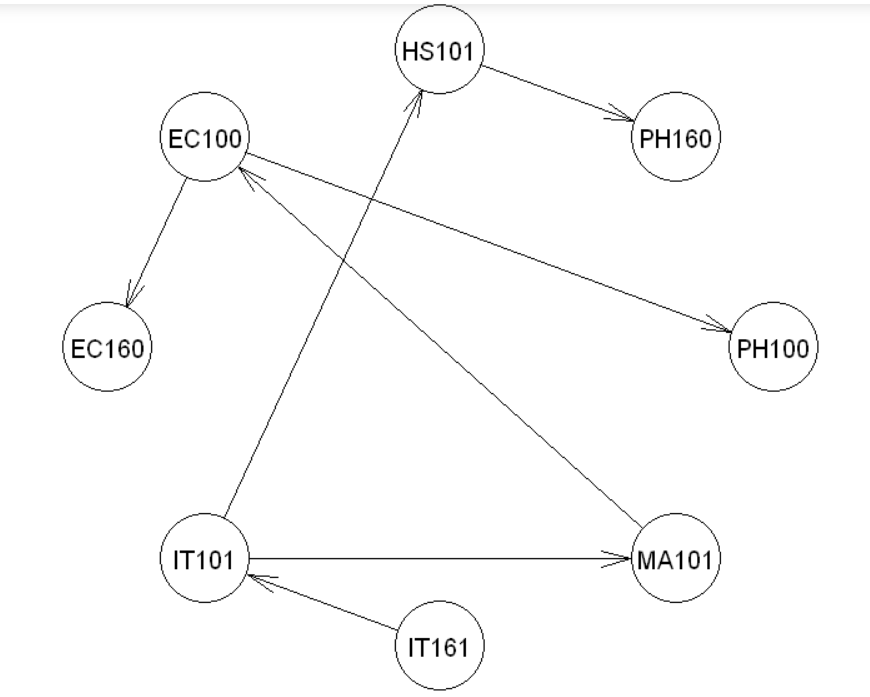
\includegraphics[width=0.48\textwidth]{images/Bayesian_K2.png}
\caption{Hill Climbing with k2 Score} % Caption change
\label{fig:ecg}
\end {center}
\end{figure}

MODEL: There are 7 dependencies between each subject which can seen from the above fig. using k2 score and the dependencies are
[IT161][IT101|IT161][MA101|IT101][HS101|IT101]
[EC100|MA101][PH160|HS101][EC160|EC100]
[PH100|EC100]

\subsection{Using the data, learn the CPTs for each course node.}


Using hill climbing K2 score the CPTs of each course is plotted below:\\

%% Figure Baki


\begin{figure}[H]%[!ht]
\begin {center}
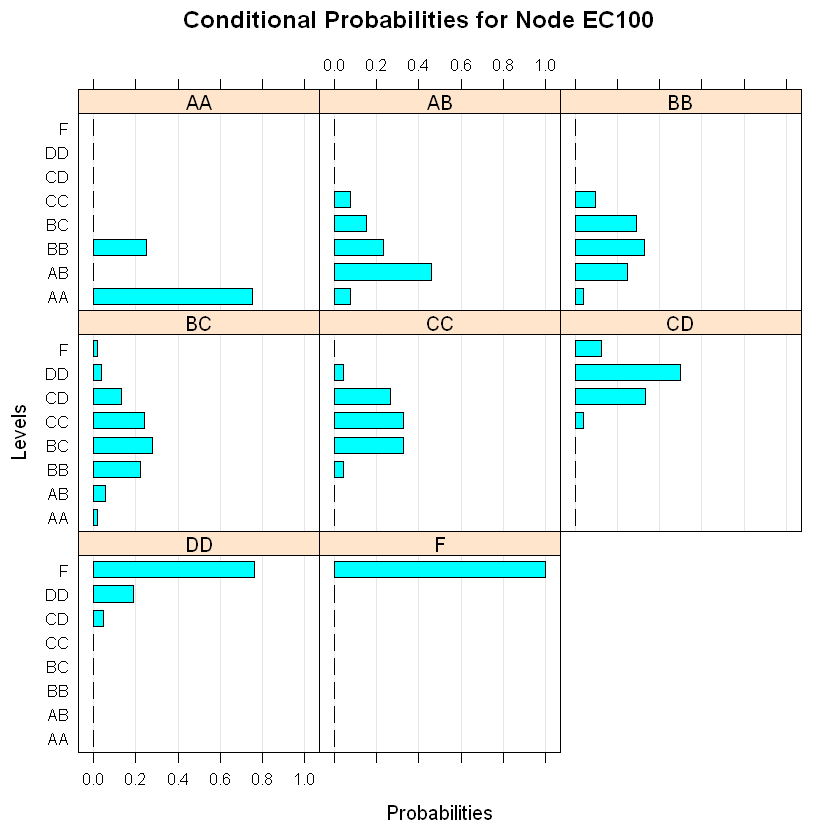
\includegraphics[width=0.48\textwidth]{images/EC100.png}
\caption{CPT of EC100} % Caption change
\label{fig:ecg}
\end {center}
\end{figure}

\begin{figure}[H]%[!ht]
\begin {center}
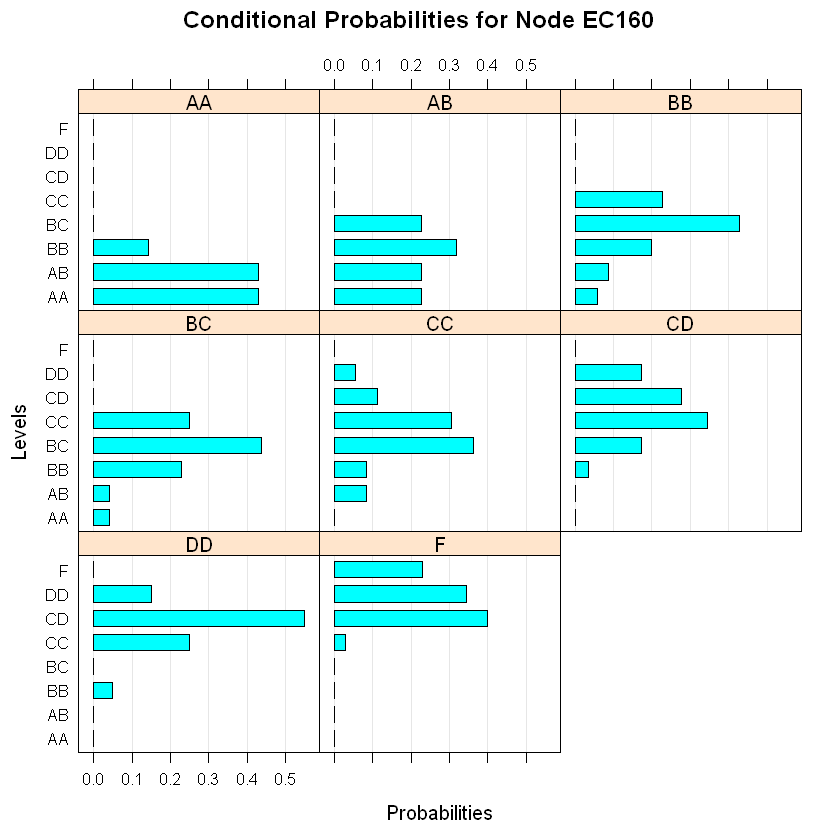
\includegraphics[width=0.48\textwidth]{images/EC160.png}
\caption{CPT of EC100} % Caption change
\label{fig:ecg}
\end {center}
\end{figure}

\begin{figure}[H]%[!ht]
\begin {center}
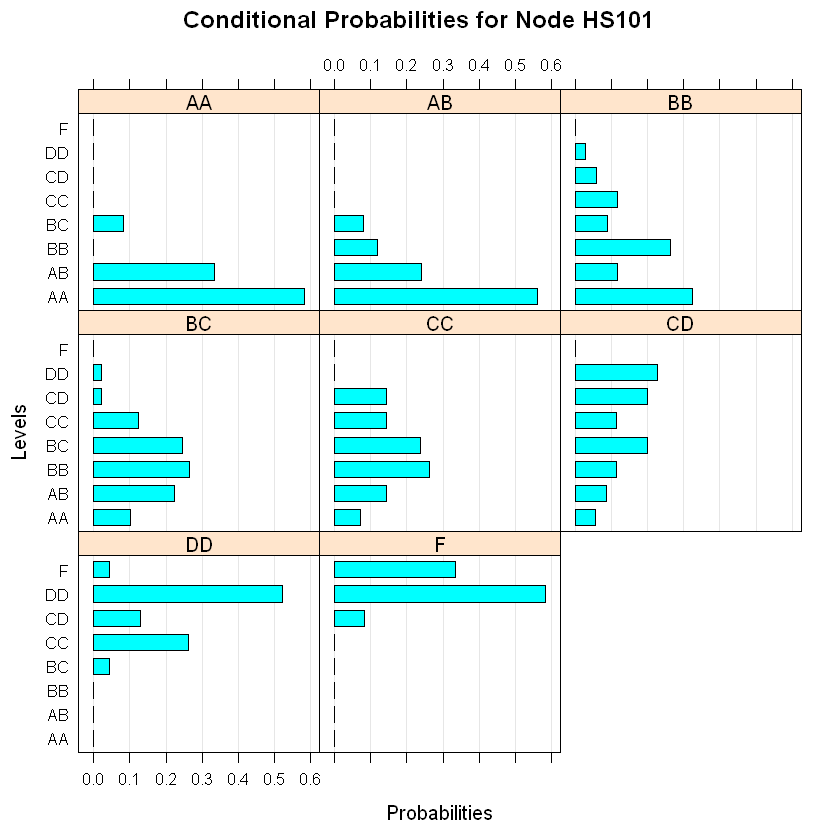
\includegraphics[width=0.48\textwidth]{images/hs101.png}
\caption{CPT of EC100} % Caption change
\label{fig:ecg}
\end {center}
\end{figure}

\begin{figure}[H]%[!ht]
\begin {center}
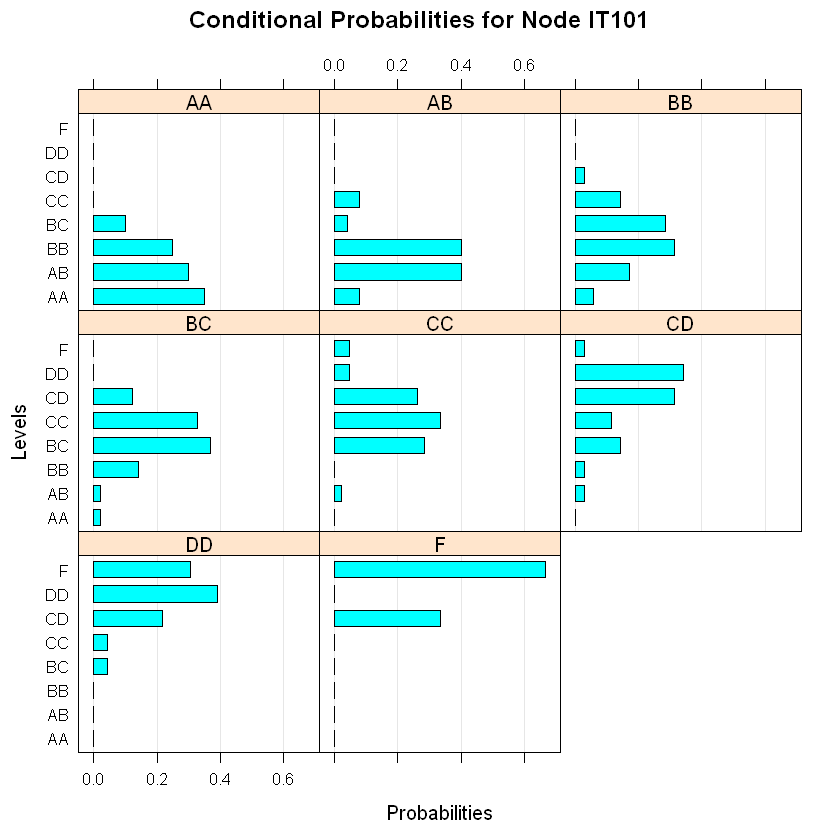
\includegraphics[width=0.48\textwidth]{images/IT101.png}
\caption{CPT of EC100} % Caption change
\label{fig:ecg}
\end {center}
\end{figure}

\begin{figure}[H]%[!ht]
\begin {center}
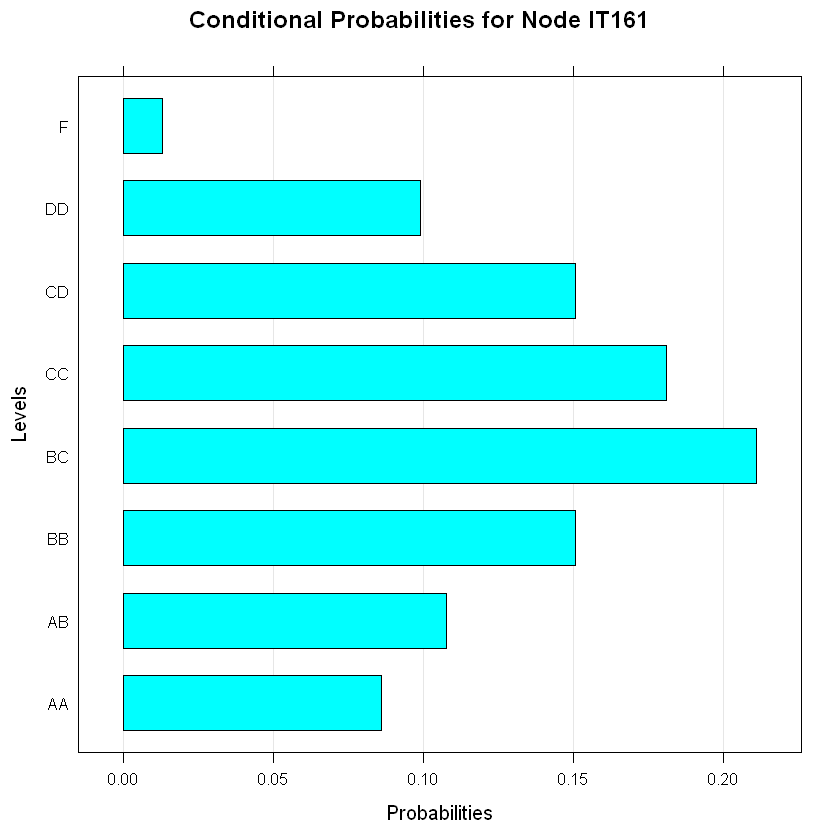
\includegraphics[width=0.48\textwidth]{images/IT161.png}
\caption{CPT of EC100} % Caption change
\label{fig:ecg}
\end {center}
\end{figure}

\begin{figure}[H]%[!ht]
\begin {center}
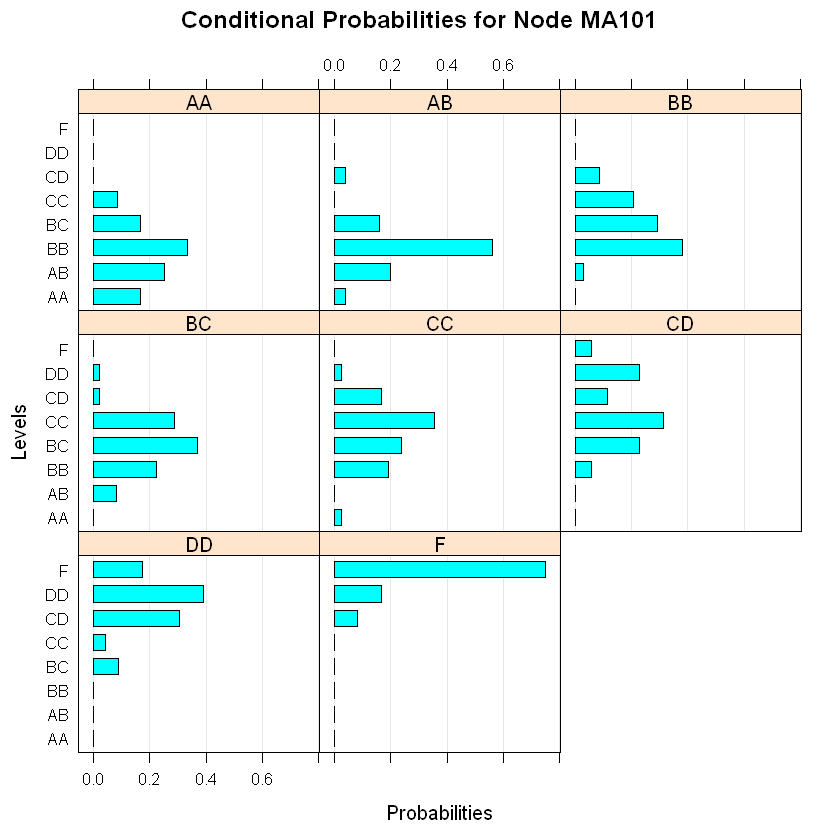
\includegraphics[width=0.48\textwidth]{images/MA101.png}

\caption{CPT of EC100} % Caption change
\label{fig:ecg}
\end {center}
\end{figure}

\begin{figure}[H]%[!ht]
\begin {center}
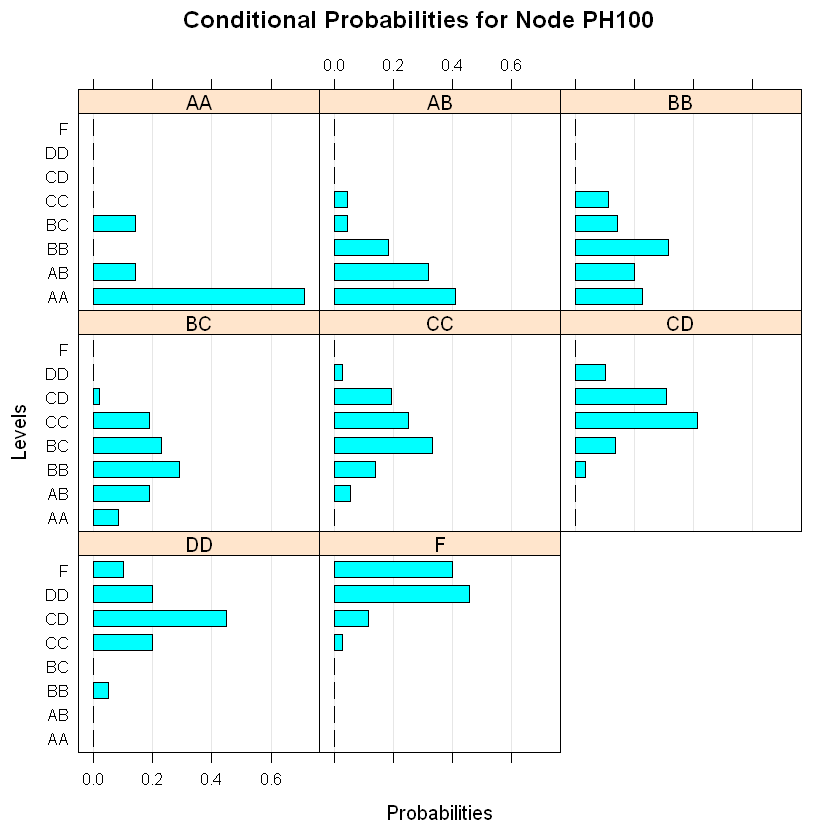
\includegraphics[width=0.48\textwidth]{images/PH100.png}
\caption{CPT of EC100} % Caption change
\label{fig:ecg}
\end {center}
\end{figure}

\begin{figure}[H]%[!ht]
\begin {center}
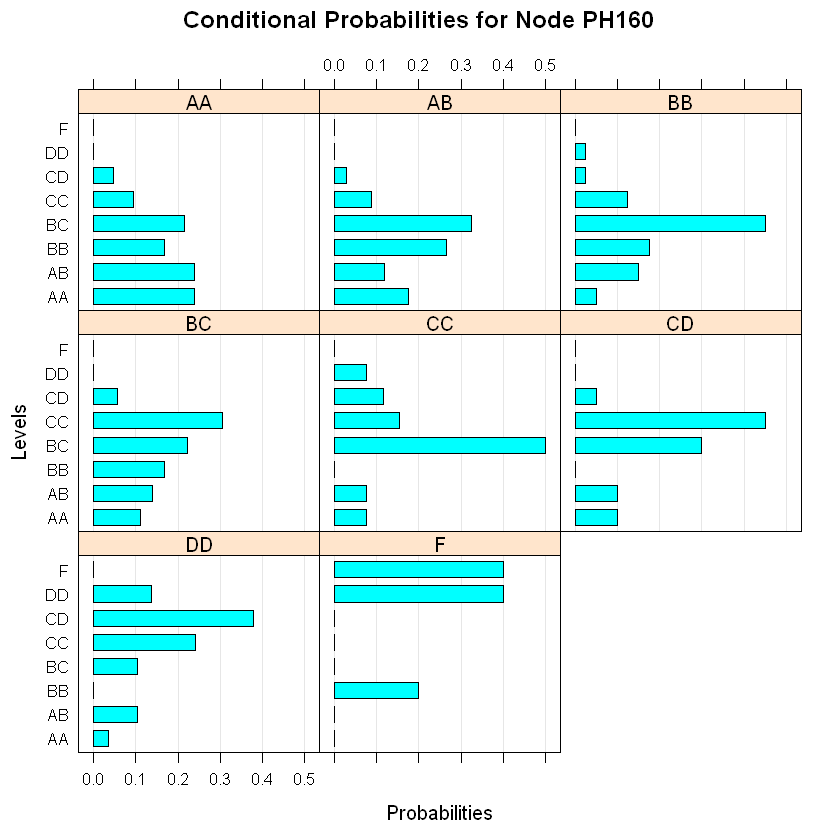
\includegraphics[width=0.48\textwidth]{images/PH160.png}
\caption{CPT of EC100} % Caption change
\label{fig:ecg}
\end {center}
\end{figure}


\subsection{What grade will a student get in PH100 if he arns DD in EC100, CC in IT101 and CD in MA101.Any of this trained model would give the same prediction about the grade}
\underline{Answer:}
We use cpquery method for getting the value that match with given condition. After applying method it is most likely to 'DD' grade in PH100

\subsection{The last column in the data file indicates whether a student qualifies for an internship program or not. From the given data, take 70 percent data for training and build a naive Bayes classifier (considering that the grades earned in different courses are independent of each other) which takes in the student’s performance and returns the qualification status with a probability. Test your classifier on the remaining 30 percent data. Repeat this experiment for 20 random selection of training and testing data. Report results about the accuracy of your classifier.}

\underline{Answer:}
This networks works on splited data which we have use-in for training the model.In the second case, dependencies to exits among courses as well with QP through an direct acyclic graph(DAG).We here use Naive Bayes network from bnclassify. The structure is shown below:
\begin{figure}[H]%[!ht]
\begin {center}
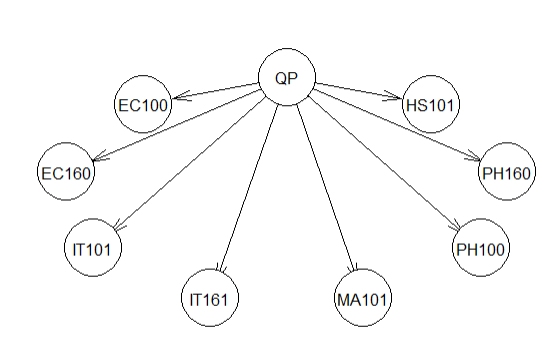
\includegraphics[width=0.48\textwidth]{images/naive (2).png}
\caption{Naive Bayes Independent data} % Caption change
\label{fig:ecg}
\end {center}
\end{figure}

This network learns on the training dataset that we split before and test it on test data.The Table below shows the accuracy:
\begin{table}[!ht] %[H]
\centering
\begin{tabular}{| c | c |}
\hline
Experiment No. &  Accuracy \\
\hline 
1 & 0.987013  \\
\hline
2 & 0.974026 \\
\hline
3 & 0.987013 \\
\hline
4 & 0.974026  \\
\hline
5 & 0.987013  \\
\hline
6 & 0.974026 \\
\hline
7 & 0.987013 \\
\hline
8 & 0.9871795 \\
\hline
9 & 0.961039 \\
\hline
10 & 0.9615385 \\
\hline
11 & 0.9871795 \\
\hline
12 & 0.974026 \\
\hline
13 & 0.987013 \\
\hline
14 & 1 \\
\hline
15 & 0.987013 \\
\hline
16 & 0.974026 \\
\hline
17 & 1 \\
\hline
18 & 0.974026 \\
\hline
19 & 0.987013 \\
\hline
20 & 0.974026 \\
\hline
\end{tabular}

\label{table:Exps}
\caption{Accuracy on test dataset on Naive Bayes classifier in independent data}
\end{table}

\subsection{Repeat 4, considering that the grades earned in different courses may be dependent.}
% Figure left

\underline{Answer:}
\begin{figure}[H]%[!ht]
\begin {center}
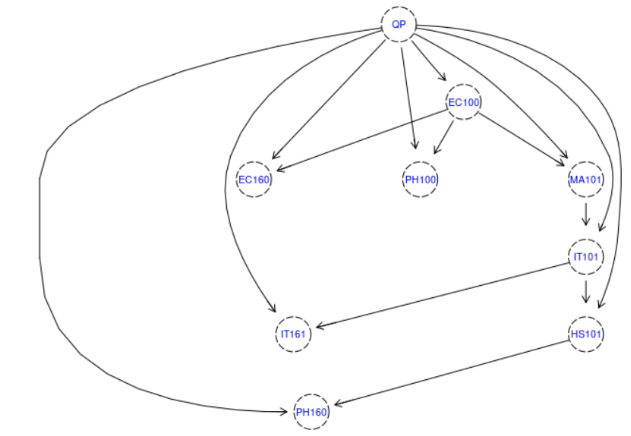
\includegraphics[width=0.48\textwidth]{images/Q5.png}
\caption{Naive Bayes dependent data} % Caption change
\label{fig:ecg}
\end {center}
\end{figure}



\begin{table}[!ht] %[H]
\centering
\begin{tabular}{| c | c |}
\hline
Experiment No. &  Accuracy \\
\hline 
1 & 0.8974359  \\
\hline
2 & 0.961039 \\
\hline
3 & 0.9358974 \\
\hline
4 & 0.974359  \\
\hline
5 & 0.9473684  \\
\hline
6 & 0.9487179 \\
\hline
7 & 0.9480519 \\
\hline
8 & 0.9480519 \\
\hline
9 & 0.974026 \\
\hline
10 & 0.9615385 \\
\hline
11 & 0.9342105 \\
\hline
12 & 0.9358974 \\
\hline
13 & 0.9480519 \\
\hline
14 & 0.9480519 \\
\hline
15 & 0.9487179 \\
\hline
16 & 0.9220779 \\
\hline
17 & 0.8961039 \\
\hline
18 & 0.9615385 \\
\hline
19 & 0.9868421 \\
\hline
20 & 0.9342105 \\
\hline
\end{tabular}

\label{table:Exps}
\caption{Accuracy on test dataset on Naive Bayes classifier in dependent data}
\end{table}

%%%%%%%%%%%%%%%%%%%%%%%%%%%%%SECOND HALF%%%%%%%%%%%%%%%%%%%%%%%%%%%%%%%%%%

\section{\large{\underline{WEEK 10}}}
Basic of data structure needed for state-space search tasks and use of random numbers required for MDP and RL

\subsection{Read the reference on MENACE by Michie and check for its implementations.  Pick the one that you like the most and go through the code carefully.  Highlight the parts that you feel are crucial.  If possible, try to code the MENACE in any programming language of your liking.}
\underline{Answer:} 
MENACE(Matchbox Educable Noughts and Crosses Engine) is a simple machine learning system(based on trail and error) designed to learn tic-tac-toe. It was developed by Donald Michie in 1961-62. He used a total 304 matchboxes, on which he drew almost all possible states or position of game. Each box contains colored beads, where each blank space is assigned with a different color bead. While playing the game, he decided to have rewards i.e if the MENACE wins then three beads of same color corresponding to the moves are being added by backtracking the moves. If the MENACE loses the game, then MENACE is punished by removing beads of same color corresponding to the moves are being removed using same backtracking method. Here there a province for the game having to be drawn, where single bead of same color corresponding to the move is being added. The MENACE move at the starting of the game is chosen randomly, and according to that further game is carried out. After many games the MENACE based upon rewards received will be trained and will be capable to win against a human. Code for the MENACE is present in the GitHub repository.
\emph{Resources:} \href{https://people.csail.mit.edu/brooks/idocs/matchbox.pdf}{menace}



%%%%%%%%%%%%%%%ADD NEW%%%%%%%%%%%%%%%%%%%%%%%%%%%%%%%%%%%%%%
\section{\large{\underline{WEEK 11}}}
Understanding Exploitation - Exploration in simple n-arm bandit reinforcement learning task, epsilon-greedy algorithm

\subsection{Consider a binary bandit with two rewards {1-success, 0-failure}.  The bandit returns 1 or 0 for the action that you select, i.e. 1 or 2.  The rewards are stochastic (but stationary).  Use an epsilon-greedy algorithm discussed in class and decide upon the action to take for maximizing the expected reward.  There are two binary bandits named binaryBanditA.m and binaryBanditB.m are waiting for you.}
\underline{Answer:}
After using both the rewards(function) binaryBanditA and
binaryBanditB here are the observations :

When the probability of rewards was low (for banditA), the expected rewards were 0 at first, but as the number of trials increased, the expected rewards increased as well. However, in the case of banditB, because the reward probability was high (0.8 and 0.9), the expected payouts in the beginning were near to 1, and when the steps were increased, the expected rewards became constant due to the averaging factor.


\begin{figure}[H]%[!ht]
\begin {center}
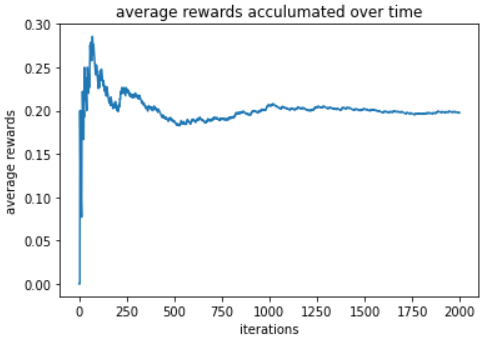
\includegraphics[width=8cm]{images/lab9_1.PNG}
\caption{Expected rewards we get after using banditA} 
\label{fig:ecg}
\end {center}
\end{figure}






\begin{figure}[H]%[!ht]
\begin {center}
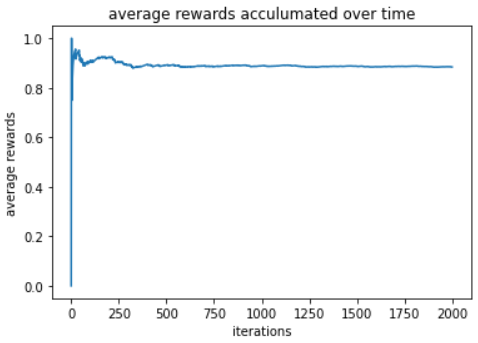
\includegraphics[width=7.7cm]{images/lab9_2.PNG}
\caption{Expected rewards we get after using banditB} 
\label{fig:ecg}
\end {center}
\end{figure}


\subsection{Develop a 10-armed bandit in which all ten mean-rewards start out equal and then take independent random walks (by adding a normally distributed increment with mean zero and standard deviation 0.01 to all mean-rewards on each time step). 
    {function [value] = bandit_nonstat(action)}}

\underline{Answer:}
The mean-rewards are initially taken as a constant valued array initialised by 1 in the case of a ten-arm bandit. We performed exploration and exploitation based on the
Epsilon Greedy Algorithm.  We produce a random number between 0 and 1, and if it is greater than epsilon, we perform exploitation, which is based on prior knowledge.
Every iteration generates a ten-value array that is normally distributed with a mean of zero and a standard deviation of 0.01. This array is added to the mean array, and this updated array is used every time. For every action a reward is given from this updated mean-rewards array. The rewards given in this case are non-stationary.


\begin{figure}[H]%[!ht]
\begin {center}
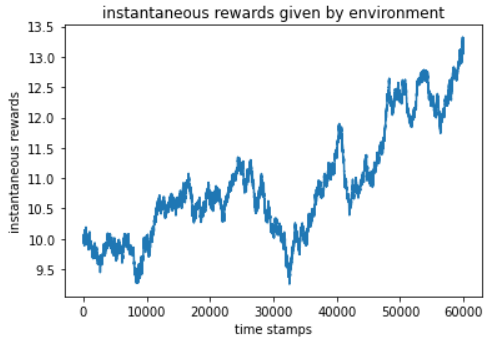
\includegraphics[width=7.7cm]{images/lab9__3.PNG}
\caption{Expected rewards we get when rewards are non
stationary (averaging method)} 
\label{fig:ecg}
\end {center}
\end{figure}




We can see that because all the rewards were initially equal to 0, we obtain a constant reward of say 1, but as the steps increase, it affects the rewarding policy of every action, and therefore the expected rewards started increasing at a very high non-zero rate.

\subsection { The 10-armed bandit that you developed is difficult to crack with a standard epsilon-greedy algorithm since the rewards are non-stationary.  We did discuss how to track non-stationary rewards in class.  Write a modified epsilon-greedy agent and show whether it is able to latch onto correct actions or not.  (Try at least 10000 time steps before commenting on results)}
\underline{Answer:}
The main difference between this problem and Problem 2 is that in Problem 2, an average method was used to update the action reward estimation, but in this problem, more weight is given to current earned reward by using the alpha parameter.

\begin{figure}[H]%[!ht]
\begin {center}
\includegraphics[width=8cm]{images/lab9_4.PNG}
\caption{Expected rewards we get when rewards are non
stationary (averaging method)} 
\label{fig:ecg}
\end {center}
\end{figure}



\includegraphics[width=8cm]{images/lab9_4.PNG}

Fig. 39: Expected rewards we get when rewards are non
stationary (averaging method)

\begin{figure}[H]%[!ht]
\begin {center}
\includegraphics[width=8cm]{images/lab9_5.PNG}
\caption{Expected rewards we get when rewards are non
stationary (non averaging method)} 
\label{fig:ecg}
\end {center}
\end{figure}




\begin{figure}[H]%[!ht]
\begin {center}
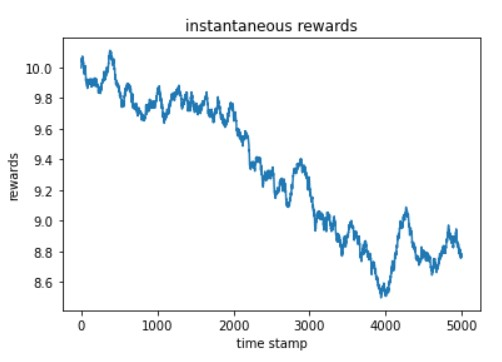
\includegraphics[width=0.45\textwidth]{images/instantous reward.jpg}
\caption{ Instantous reward} 
\label{fig:ecg}
\end {center}
\end{figure}



The expected rewards were substantially higher than in case 2, and the slope of the graph was much steeper than that in case 1.

 \emph{Resource:}
 \href{https://web.stanford.edu/class/psych209/Readings/SuttonBartoIPRLBook2ndEd.pdf}{n-bandit Problem}



%%%%%%%%%%%%%%%%%%%%%%%%%%%%%%%%%%%


\section{\large{\underline{WEEK 13}}}
To understand the design of type-1 (Mamdani) Fuzzy expert system

In this laboratory, we will try to identify the appropriate time needed to wash the load of clothes, given the dirtiness and the volume of the load.  This is a simplified design, in practice a lot more variables are involved including: water level, amount of detergent to be dispensed, and temperature of water (recent development) and variables that you and I may imagine in future.

A simple rule-base for the washing machine time problem is given below for reference.

\begin{table}[]
\begin{tabular}{lllll}
 &Load Dirtiness/ Load Volume  &vd  &md  &ld &nd  \\
 &  &  &  &  \\
 &  &  &  &  \\
 &  &  &  & 
\end{tabular}
\end{table}

\subsection{The rule table consists of 12 rules.}

If	load volume 	is	medium load\\
And	load dirtiness	is	lightly dirty\\
Then	washing time	is	medium time\\

\underline{Answer:} 
;We examine a simple two-input one-output
problem that includes total 12 rules using Mamdami-style
fuzzy inference process\\
input : x and y (Load Dirtiness and Load Volume) with
linguistic values A1,A2,A3,A4 (very dirty,medium dirty,low
dirty,not dirty) and B1,B2,B3 (full load,medium load,low
load) respectively\\
Output: z (time needed) with linguistic values C1,C2,C3,
and C4 (very long time,long time,medium time and little
time).\\
Let’s define membership functions for all input linguistic
value (i.e., for A1)
membership function for Load Dirtiness\\
 \mu_{A1(x)} = (x−60)/40, 60 $\leq$ x $\leq$ 100
   %%%%change
  

   \mu_{A2(x)} = (65-x)/15, 50 $\leq$ x $\leq$ 65
   

   \mu_{A3(x)} = (35-x)/15, 20 $\leq$ x $\leq$35
   

   \mu_{A4(x)} = (5-x)/5, 0 $\leq$ x $\leq$ 5

membership function for Load Volume\\
 \mu_{B1(x)} = (x−50)/50, 50 $\leq$ x $\leq$ 100
   %%%%change
  

   \mu_{B2(x)} = (100-x)/50, 50 $\leq$ x $\leq$ 100
   

   \mu_{B3(x)} = (50-x)/50, 0$\leq$ x $\leq$50\\%%
   
  
\textbf{Step 1: Fuzzification}\\

\begin{enumerate}
    \item Take the crisp inputs, x1 and y1 (Load Dirtiness and Load Volume)
    \item Determine the degree to which these inputs belong to each of the appropriate fuzzy sets.
\end{enumerate}
   
\textbf{Step 2: Rule Evaluation }\\

Take the fuzzified inputs, and apply them to the antecedents of the fuzzy rules. If a given fuzzy rule has multiple antecedents, the fuzzy operator (AND or OR) is used to obtain a single number that represents the result of the antecedent evaluation. This number (the truth value) is then applied to the consequent membership function.
For example, the entry in the second row and the third column of the table specifies the rule:\\
If load volume (y) is medium load (B1)\\
\textbf{AND} load dirtiness (x) is low dirty (A3)
Then washing time is medium time
and for x1 = 91, y1 = 79\\
\begin{equation}
    \mu_{A3\cap B1} (x) = min[\mu_{A3},\mu_{B1}]   = min(0,0.58)=0 
\end{equation}

\textbf{OR}
\begin{equation}
    \mu_{A3\cap B1} (x) = prod[\mu_{A3},\mu_{B1}]   = \mu_{A3} x \mu_{B1} = 0x0.58 =0 
\end{equation}

The result of the antecedent evaluation can be applied to the membership function of the consequent. In other words, the consequent membership function is clipped or scaled to the level of the truth value of the rule antecedent\\

\textbf{Step 3 Aggregation of the rule outputs} the membership functions of all rule consequent previously clipped or scaled and combine them into a single fuzzy set.

\textbf{Step 4 Defuzzification} Centroid Technique: Here we find the centroid of the found  model using the below formula:



\begin{equation}
COG = \frac{\int_a^b\!uA(x)x\, \mathrm{d}x}{\int_a^b\!uA(x)\, \mathrm{d}x}
\label{eq:cogCont}
\end{equation}


\emph{Resources:} \href{http://www.cs.utsa.edu/~bylander/cs5233/a-b-analysis.pdf}{Fuzzy Expert system}




\section{{Link for Laboratory code}}
The complete codes for different Laboratories is given below:
\href{https://github.com/rakshil14-2/AI-LabCodes}{GitHub}







\end{document}


